\documentclass[a4paper,11pt]{report}
\usepackage{chuan_math_gkt}
\usetikzlibrary{angles,quotes,intersections,patterns,decorations.pathreplacing}
\chuanexamsetup

\begin{document}
\examfontsize

\examsecret{绝密$\bigstar$启用前}

\examtitle{2021年普通高等学校招生全国统一考试（全国乙卷文科）}{数\quad 学}

\noticetitle
\begin{examnotice}
\item 答卷前，考生务必将自己的姓名、准考证号填写在答题卡上。
\item 回答选择题时，选出每小题的答案后，用铅笔把答题卡上对应题目的答案标号涂黑。如需改动，用橡皮擦干净后，再选涂其他答案标号。回答非选择题时，将答案写在答题卡上。写在本试卷上无效。
\item 考试结束后，将本试卷和答题卡一并交回。
\end{examnotice}
\examsection{一、选择题：本题共12小题，每小题5分，共60分。在每小题给出的四个选项中，只有一项是符合题目要求的。}
\begin{examquestions}

\item 已知全集$U=\{1,2,3,4,5\}$，集合$M=\{1,2\}$，$N=\{3,4\}$，则$C_{U}(M\cup N)=$（
)

\fourchoices{$\{5\}$}{$\{1,2\}$}{$\{3,4\}$}{$\{1,2,3,4\}$}

\item 设$iz=4+3i$，则$z=$

\fourchoices{$-3-4i$}{$–3+4i$}{$3-4i$}{$3+4i$}

\item 已知命题$p:∃x\ensuremath{\in} R,sinx<1$；命题$q:∀x\ensuremath{\in} R,e^{|x|}\ensuremath{\geq}1$，则下列命题中为真命题的是

\fourchoices{$p∧q$}{$¬p∧q$}{$p∧¬q$}{$¬(p∨q)$}

\item 函数$f(x)=\sin\dfrac{x}{3}+\cos\dfrac{x}{3}$的最小正周期和最大值分别是

\fourchoices{$3\pi$和$\sqrt{2}$}{$3\pi$和$2$}{$6\pi$和$\sqrt{2}$}{$6\pi$和$2$}

\item 若$x,y$满足约束条件\linsys{x+y\ensuremath{\geq}4,\\x-y\ensuremath{\leq}2,\\y\ensuremath{\leq}3,}则$z=3x+y$的最小值为

\fourchoices{$18$}{$10$}{$6$}{$4$}

\item $\cos^2\dfrac{\pi}{12}-\cos^2\dfrac{5\pi}{12}=$

\onechoices{$\dfrac{1}{2}$}{$\dfrac{\sqrt{3}}{3}$}{$\dfrac{\sqrt{2}}{2}$}{$\dfrac{\sqrt{3}}{2}$}

\item 在区间$(0,\dfrac{1}{2})$随机取$1$个数，则取到的数小于$\dfrac{1}{3}$的概率为

\fourchoices{$\dfrac{3}{4}$}{$\dfrac{2}{3}$}{$\dfrac{1}{3}$}{$\dfrac{1}{6}$}

\item 下列函数中最小值为$4$的是

\onechoices{$y=x^{2}+2x+4$}{$y=|sinx|+\dfrac{4}{|sinx|}$}{$y=2^{x}+2^{2-x}$}{$y=\ensuremath{\ln x}+\dfrac{4}{\ensuremath{\ln x}}$}

\item 设函数$f(x)=\dfrac{1-x}{1+x}$，则下列函数中为奇函数的是

\fourchoices{$f(x-1)-1$}{$f(x-1)+1$}{$f(x+1)-1$}{$f(x+1)+1$}

\item 在正方体$ABCD-A_{1}B_{1}C_{1}D_{1}$中，$P$为$B_{1}D_{1}$的中点，则直线$PB$与$AD_{1}$所成的角为

\fourchoices{$\dfrac{\pi}{2}$}{$\dfrac{\pi}{3}$}{$\dfrac{\pi}{4}$}{$\dfrac{\pi}{6}$}

\item 设$B$是椭圆$C$:$\dfrac{x^{2}}{5}+y^{2}=1$的上顶点，点$P$在$C$上，则$|PB|$的最大值为

\fourchoices{$\dfrac{5}{2}$}{$\sqrt{6}$}{$\sqrt{5}$}{$2$}

\item 设$a\ne0$，若$x=a$为函数$f(x)=a(x-a)^{2}(x-b)$的极大值点，则

\fourchoices{$a<b$}{$a>b$}{$ab<a^{2}$}{$ab>a^{2}$}

\item 已知向量$\vec{a}=(2,5)$，$\vec{b}=(\lambda,4)$，若$\vec{a}//\vec{b}$，则$\lambda=$
.

\item 双曲线$\dfrac{x^{2}}{4}-\dfrac{y^{2}}{5}=1$的右焦点到直线$x+2y-8=0$的距离为
.

\item 记$\ensuremath{\triangle} ABC$的内角$A$，$B$，$C$的对边分别为$a$，$b$，$c$，面积为$\sqrt{3}$，
$B=60^\circ$,$a^{2}+c^{2}=3ac$，则$b=$
.

\item 以图①为正视图，在图②③④⑤中选两个分别作为侧视图和俯视图，组成某个三棱锥的三视图，则所选侧视图和俯视图的编号依次为
（写出符合要求的一组答案即可）.

\begin{tightcenter}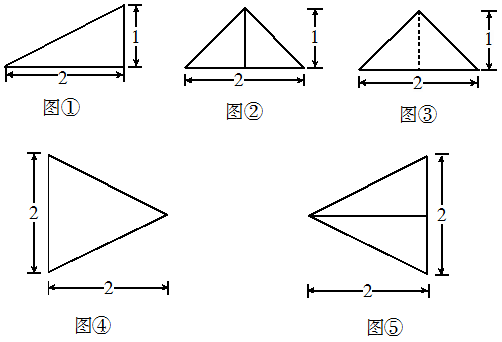
\includegraphics[width=2.70347in,height=1.84167in]{figures/2021_yi_wen_image102.png}\end{tightcenter}

\item 某厂研制了一种生产高精产品的设备，为检验新设备生产产品的某项指标有无提高，用一台旧设备和一台新设备各生产了$10$件产品，得到各件产品该项指标数据如下：

\begin{tightcenter}
\begin{tabular}{|c|c|c|c|c|c|c|c|c|c|c|}
\hline
旧设备 & 9.8 & 10.3 & 10.0 & 10.2 & 9.9 & 9.8 & 10.0 & 10.1 & 10.2 & 9.7 \\ \hline
新设备 & 10.1 & 10.4 & 10.1 & 10.0 & 10.1 & 10.3 & 10.6 & 10.5 & 10.4 & 10.5 \\ \hline
\end{tabular}
\end{tightcenter}

旧设备和新设备生产产品的该项指标的样本平均数分别记为$\overline{x}$和$\overline{y}$，样本方差分别记为$s_{1}^{2}$和$s_{2}^{2}$.

（1）求$\overline{x}$，$\overline{y}$，$s_{1}^{2}$，$s_{2}^{2}$；

（2）判断新设备生产产品的该项指标的均值较旧设备是否有显著提高（如果$\overline{y}-\overline{x}\ensuremath{\geq}2\sqrt{\dfrac{s_{1}^{2}+s_{2}^{2}}{10}}$，则认为新设备生产产品的该项指标的均值较旧设备有显著提高，否则不认为有显著提高）.

\item 如图，四棱锥$P-ABCD$的底面是矩形，$PD\ensuremath{\perp}$底面$ABCD$，$M$为$BC$的中点，且$PB\ensuremath{\perp} AM$.

（1）证明：平面$PAM\ensuremath{\perp}$平面$PBD$﹔

（2）若$PD=DC=1$，求四棱锥$P-ABCD$的体积.

\begin{tightcenter}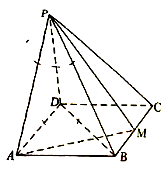
\includegraphics[width=1.67708in,height=1.77083in]{figures/2021_yi_wen_image123.png}\end{tightcenter}

\item 设$\{a_{n}\}$是首项为$1$的等比数列，数列$\{b_{n}\}$满足$b_{n}=\dfrac{na_{n}}{3}$.已知$a_{1}$，$3a_{2}$，$9a_{3}$，成等差数列.

（1）求$\{a_{n}\}$和$\{b_{n}\}$的通项公式；

（2）记$S_{n}$，和$T_{n}$分别为$\{a_{n}\}$和$\{b_{n}\}$的前$n$项和.证明：$T_{n}<\dfrac{S_{n}}{2}$.

\item 已知抛物线$C$：$y^{2}=2px(p>0)$的焦点$F$到准线的距离为$2$.

（1）求$C$的方程，

（2）已知$O$为坐标原点，点$P$在$C$上，点$Q$满足$\vec{PQ}=9\vec{QF}$，求直线$OQ$斜率的最大值.

\item 已知函数$f(x)=x^{3}-x^{2}+ax+1$.

（1）讨论$f(x)$的单调性；

（2）求曲线$y=f(x)$过坐标原点的切线与曲线$y=f(x)$的公共点的坐标.

\item 在直角坐标系$xOy$中，$\odot C$的圆心为$C(2,1)$，半径为$1$.

（1）写出$\odot C$的一个参数方程;

（2）过点$F(4,1)$作$\odot C$的两条切线.以坐标原点为极点，$x$轴正半轴为极轴建立坐标系，求这两条切线的极坐标方程.

\item 已知函数$f(x)=|x-a|+|x+3|$.

（1）当$a=1$时，求不等式$f(x)\ensuremath{\geq}6$的解集；

（2）若$f(x)>-a$，求$a$的取值范围.
\end{examquestions}


\end{document}
